\documentclass{article}
\usepackage{amsmath}
\usepackage[top=2cm, left=2cm, right=1cm, bottom=2cm]{geometry}
\usepackage{fancyhdr}
\usepackage{graphicx}
\usepackage{longtable}

\usepackage{amsmath,amssymb}
\usepackage{iftex}
\ifPDFTeX
  \usepackage[T1]{fontenc}
  \usepackage[utf8]{inputenc}
  \usepackage{textcomp} % provide euro and other symbols
\else % if luatex or xetex
  \usepackage{unicode-math} % this also loads fontspec
  \defaultfontfeatures{Scale=MatchLowercase}
  \defaultfontfeatures[\rmfamily]{Ligatures=TeX,Scale=1}
\fi
\usepackage{lmodern}
\ifPDFTeX\else
  % xetex/luatex font selection
\fi
% Use upquote if available, for straight quotes in verbatim environments
\IfFileExists{upquote.sty}{\usepackage{upquote}}{}
\IfFileExists{microtype.sty}{% use microtype if available
  \usepackage[]{microtype}
  \UseMicrotypeSet[protrusion]{basicmath} % disable protrusion for tt fonts
}{}
\makeatletter
\@ifundefined{KOMAClassName}{% if non-KOMA class
  \IfFileExists{parskip.sty}{%
    \usepackage{parskip}
  }{% else
    \setlength{\parindent}{0pt}
    \setlength{\parskip}{6pt plus 2pt minus 1pt}}
}{% if KOMA class
  \KOMAoptions{parskip=half}}
\makeatother
\usepackage{xcolor}
\usepackage{longtable,booktabs,array}
\usepackage{calc} % for calculating minipage widths
% Correct order of tables after \paragraph or \subparagraph
\usepackage{etoolbox}
\makeatletter
\patchcmd\longtable{\par}{\if@noskipsec\mbox{}\fi\par}{}{}
\makeatother
% Allow footnotes in longtable head/foot
\IfFileExists{footnotehyper.sty}{\usepackage{footnotehyper}}{\usepackage{footnote}}
\makesavenoteenv{longtable}
\usepackage{graphicx}
\makeatletter
\def\maxwidth{\ifdim\Gin@nat@width>\linewidth\linewidth\else\Gin@nat@width\fi}
\def\maxheight{\ifdim\Gin@nat@height>\textheight\textheight\else\Gin@nat@height\fi}
\makeatother
% Scale images if necessary, so that they will not overflow the page
% margins by default, and it is still possible to overwrite the defaults
% using explicit options in \includegraphics[width, height, ...]{}
\setkeys{Gin}{width=\maxwidth,height=\maxheight,keepaspectratio}
% Set default figure placement to htbp
\makeatletter
\def\fps@figure{htbp}
\makeatother
\setlength{\emergencystretch}{3em} % prevent overfull lines
\providecommand{\tightlist}{%
}
\setcounter{secnumdepth}{-\maxdimen} % remove section numbering
\ifLuaTeX
  \usepackage{selnolig}  % disable illegal ligatures
\fi
\usepackage{bookmark}
\usepackage{enumitem}

\IfFileExists{xurl.sty}{\usepackage{xurl}}{} % add URL line breaks if available
\urlstyle{same}
\hypersetup{
  hidelinks,
  pdfcreator={LaTeX via pandoc}}


\begin{document}
\pagestyle{fancy}
\fancyhf{}
\lfoot{Test ID: %%TESTID%%}
\rfoot{Page: \thepage}
\renewcommand{\footrulewidth}{0.4pt}

%%KEY%%
\clearpage

\noindent
\textbf{Instructions:} For each problem, circle the letter of the best answer.
You \textbf{must show all work} for credit. Partial credit may be awarded as appropriate.

%%QUESTIONS%%

\clearpage
\section{Free Response 1}

The function

$$
f(x)=\frac{1}{x^{2}-4}
$$

has first derivative

$$
f^{\prime}(x)=\frac{-2 x}{\left(x^{2}-4\right)^{2}}
$$

and second derivative

$$
f^{\prime \prime}(x)=\frac{6 x^{2}+8}{\left(x^{2}-4\right)^{3}}
$$

Sketch the graph of $f(x)$ after completing the following questions:

\begin{enumerate}
	\setlength{\itemsep}{0.65in}
	\item State any domain restrictions for $f(x)$
	\item Determine any critical points of $f(x)$
	\item State intervals on which $f(x)$ is increasing or decreasing
	\item State intervals on which $f(x)$ is concave up or concave down
	\item Calculate any horizontal asymptotes of $f(x)$
\end{enumerate}
\vspace{0.5in}
\begin{center}
\includegraphics*[width=3in]{media/grid.png}
\end{center}

\clearpage
\section{Free Response 2}

The graph $f'(x)$  of the derivative of $f(x)$ is shown below. $f'(x)$ has horizontal tangents at $x=-2,2,4$ and zeros at $x=-4,0,4$.
The domains of $f'(x)$ and $f(x)$ are $[-6,6]$.

\begin{center}
	\includegraphics[width=4in]{media/g.png}
\end{center}

\begin{enumerate}
	\setlength{\itemsep}{1in}
	\item On which $x$ intervals is the function $f$ increasing? Justify your answer.
	\item At which $x$ value(s) does $f$ have a local maximum? Justify your answer.
	\item On which $x$ intervals is the function $f$ concave down? Justify your answer.
\end{enumerate}


\end{document}
